\addcontentsline{toc}{chapter}{\textbf{Anexo 1}} 
\lhead{Anexo 1}
\rhead{\newtitle}
\cfoot{\thepage}
\renewcommand{\headrulewidth}{1pt}
\renewcommand{\footrulewidth}{1pt}
\chapter*{Anexo 3}
\noindent En este anexo se incluyen cada una de las publicaciones que se han realizado en el transcurso de esta tesis.

\begin{itemize}
\item Salazar, G. A., Alonso-Suárez, R., Laguarda Cirigliano, A., \& Ledesma, R. D. (2022). Evaluación del proceso de adaptación al sitio aplicado a la irradiancia solar global medida en la ciudad de Salta, Argentina. Avances En Energías Renovables Y Medio Ambiente - AVERMA, 25, 353–362. 
\item Ledesma, R. D., Salazar, G. A., \& de Castro Vilela, O. (2022). Aplicación móvil como herramienta para la evaluación de modelos de irradiancia solar. En Acta de la XLIV Reunión de Trabajo de la Asociación Argentina de Energías Renovables y Ambiente (Vol. 9, pp. 186–195). ISBN 978-987-29873-1-2.

\item Ledesma, R. D., Salazar, G. A., \& de Castro Vilela, O. (2022). ARGP-V2: Un modelo práctico para la estimación de irradiancia global horizontal en condiciones de cielo claro para sitios de altura. Avances en Energías Renovables y Medio Ambiente, 26, 283–289. ISSN 2796-8111. ASADES 2022.

\item Ledesma, R., Alonso-Suárez, R., Monetta, A., Laguarda, A., Vilela, O., \& Salazar, G. (2024). Evaluación en Uruguay del producto DSR GOES-16 de irradiancia solar global horizontal. Avances En Energías Renovables Y Medio Ambiente - AVERMA, 27, 474–483.

\item Ledesma, R., Salazar, G., \& Vilela, O. (2024). Avances en la estimación de irradiancia solar en las provincias de Salta y jujuy mediante imágenes satelitales GOES-16. Avances En Energías Renovables Y Medio Ambiente - AVERMA, 27, 413–427.

\item Salazar, G., Ledesma, R. D., López Ruiz, C. ., \& de Castro Vilela, O. (2025). Análisis de desempeño de diferentes técnicas de aprendizaje automático en una adaptación al sitio de irradiancia solar global para Salta (Argentina). Avances En Energías Renovables Y Medio Ambiente - AVERMA, 28, 308–320.

\item López Ruiz, C. B., Salazar, G. A., Ledesma, R., \& Bezerra Galdino, J. J. (2025, marzo). Análisis de radiación solar difusa medida usando banda sombreadora: Caso de estudio en la ciudad de Salta. En Acta de la XLVI Reunión de Trabajo de la Asociación Argentina de Energías Renovables y Ambiente (Vol. 11, pp. 236–248). ISBN 978-987-29873-1-2.


\item Salazar, G., Ledesma, R., López Ruiz, C., \& Castro Vilela, O. (2024). Development of a solar irradiance cloud index model for Northwest Argentina using GOES-16 imagery: Comparison against reanalysis and satellite databases. En International Academy of Astronautics (Ed.), Proceedings of the International Academy of Astronautics Latin American Conference on Small Satellite Technologies and Applications (1.ª ed., pp. 191-197). International Academy of Astronautics. ISBN 978-2-917761-85-4.

\item Ledesma, R., Alonso-Suárez, R., Salazar, G., Nollas, F., \& Vilela, O. (2025). Evaluation of satellite and reanalysis models for solar irradiance estimation in Northwest Argentina. IEEE Latin America Transactions, 23(8), 706–717. https://doi.org/10.1109/TLA.2025.11072498.

\item Silvero, C. I., Forciniti, J. D., Medina, F. D., Vega Caro, M. A., Ledesma, R. D., Zossi, B. S., Mansilla, G. A., and Elias, A. G. (October 10, 2025). "Comparative Study of Solar Radiation Measurements in Tucuman, Argentina, With Reanalyses and Satellite-Based Datasets." ASME. J. Sol. Energy Eng. December 2025; 147(6): 061012.

\item Ledesma, R., Salazar, G.. (2025). Machine learning for site adaptation of satellite-derived solar irradiance in Northwestern Argentina. Journal of Computer Science and Technology, 25(2), e10. https://doi.org/10.24215/16666038.25.e10
\item Cinco Reynaga, P., \& Ledesma, R. D. (en prensa). Evaluación de algoritmos de aprendizaje automático para la clasificación de días de cielo claro. En Actas de la XLVI Reunión de Trabajo de la Asociación Argentina de Energías Renovables y Ambiente (AVERMA) (Vol. 11, pp. 236–248). ISBN 978-987-29873-1-2.
\end{itemize}
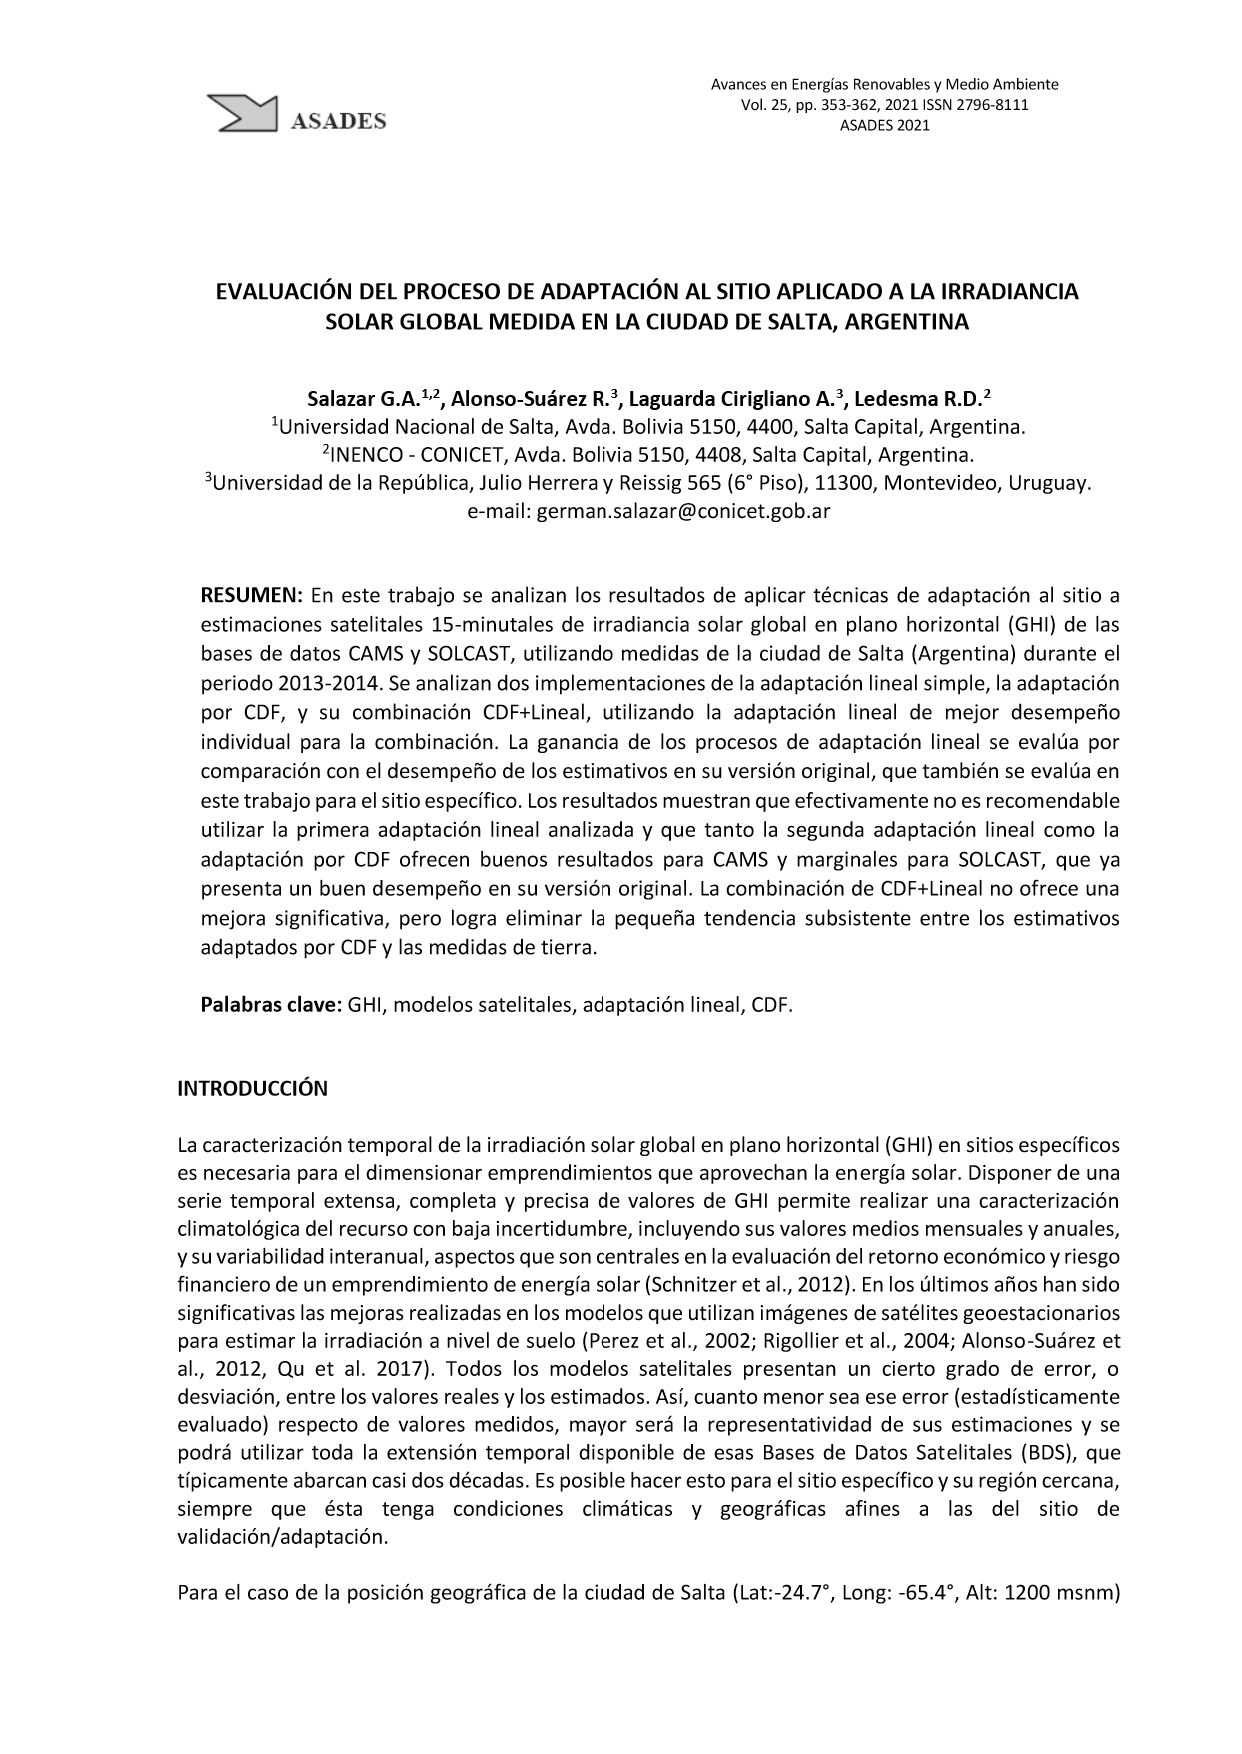
\includepdf[pages=-]{anexo_3/01_site_adaptation2}
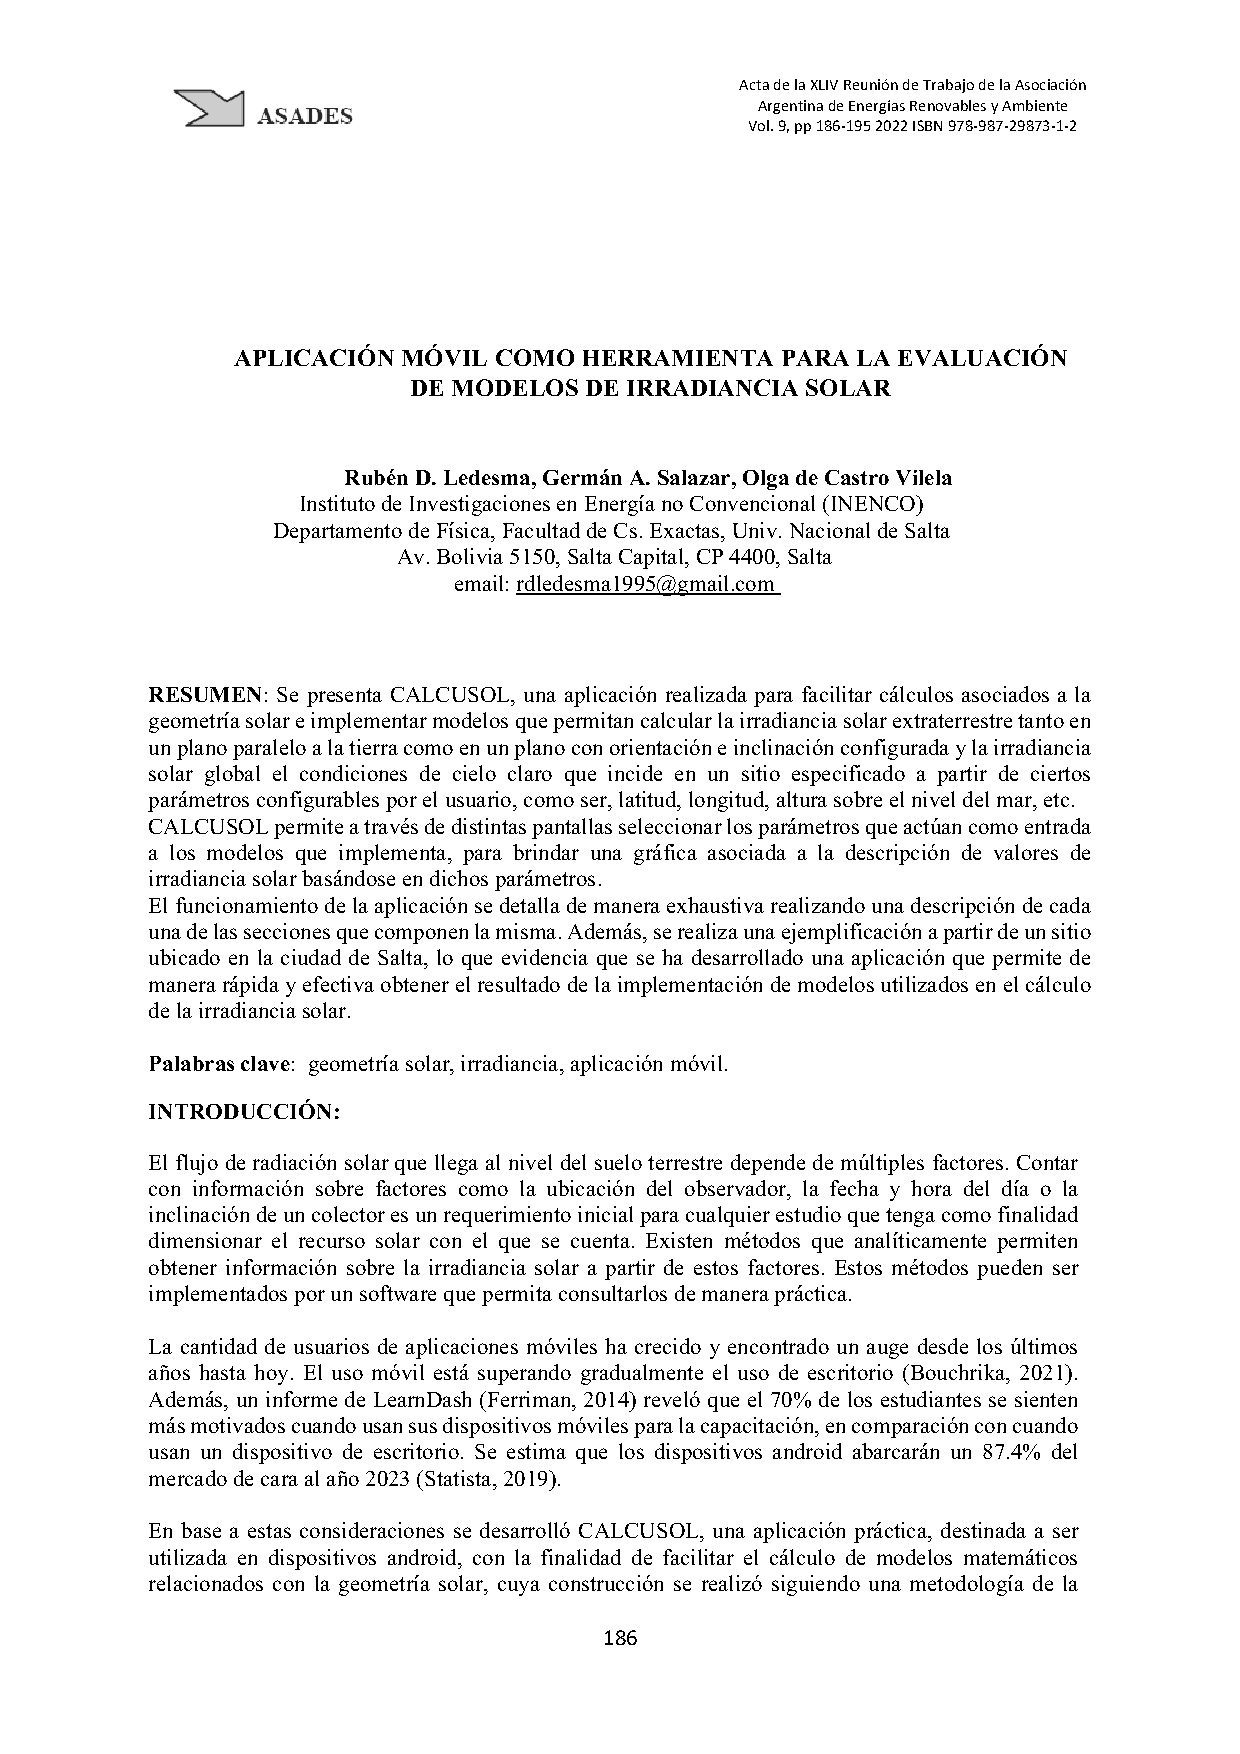
\includepdf[pages=-]{anexo_3/02_Calcusol}
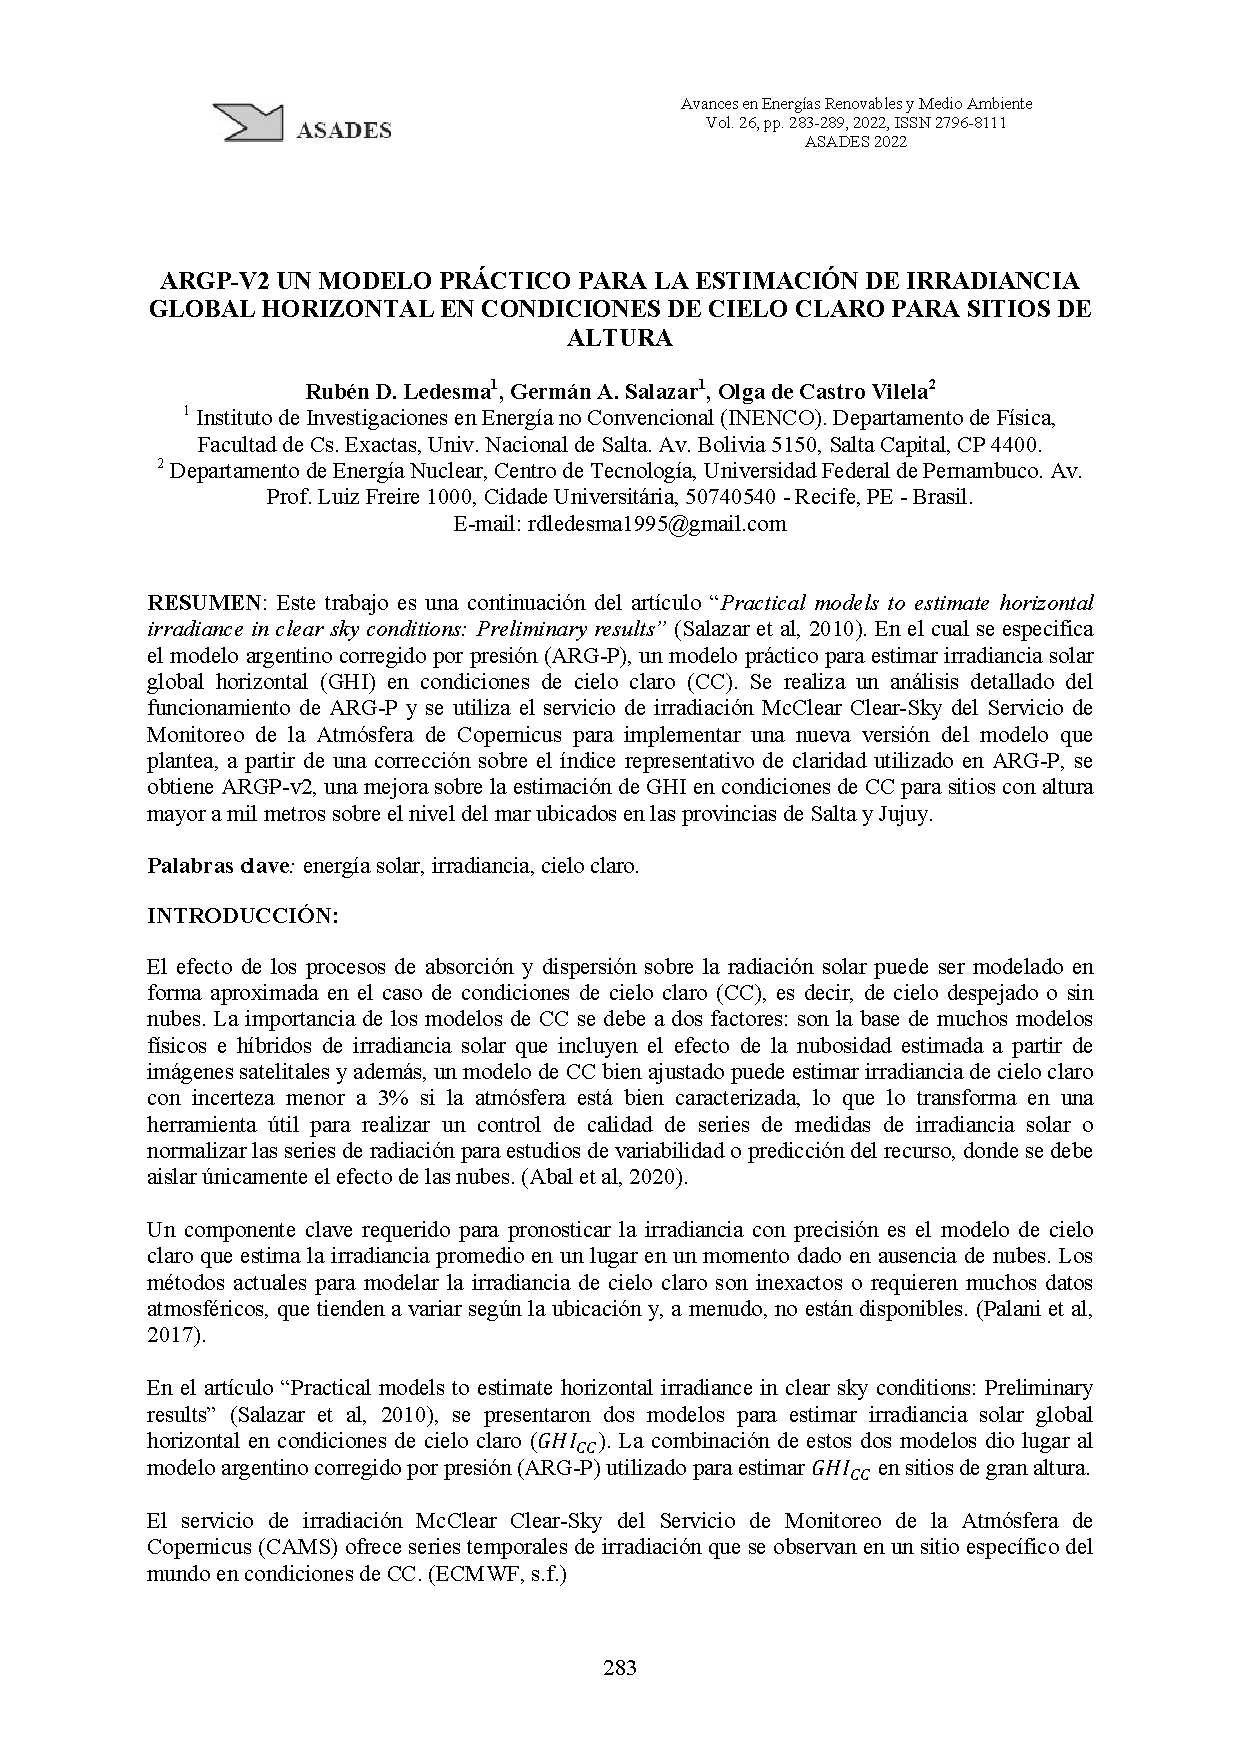
\includepdf[pages=-]{anexo_3/03_argp}
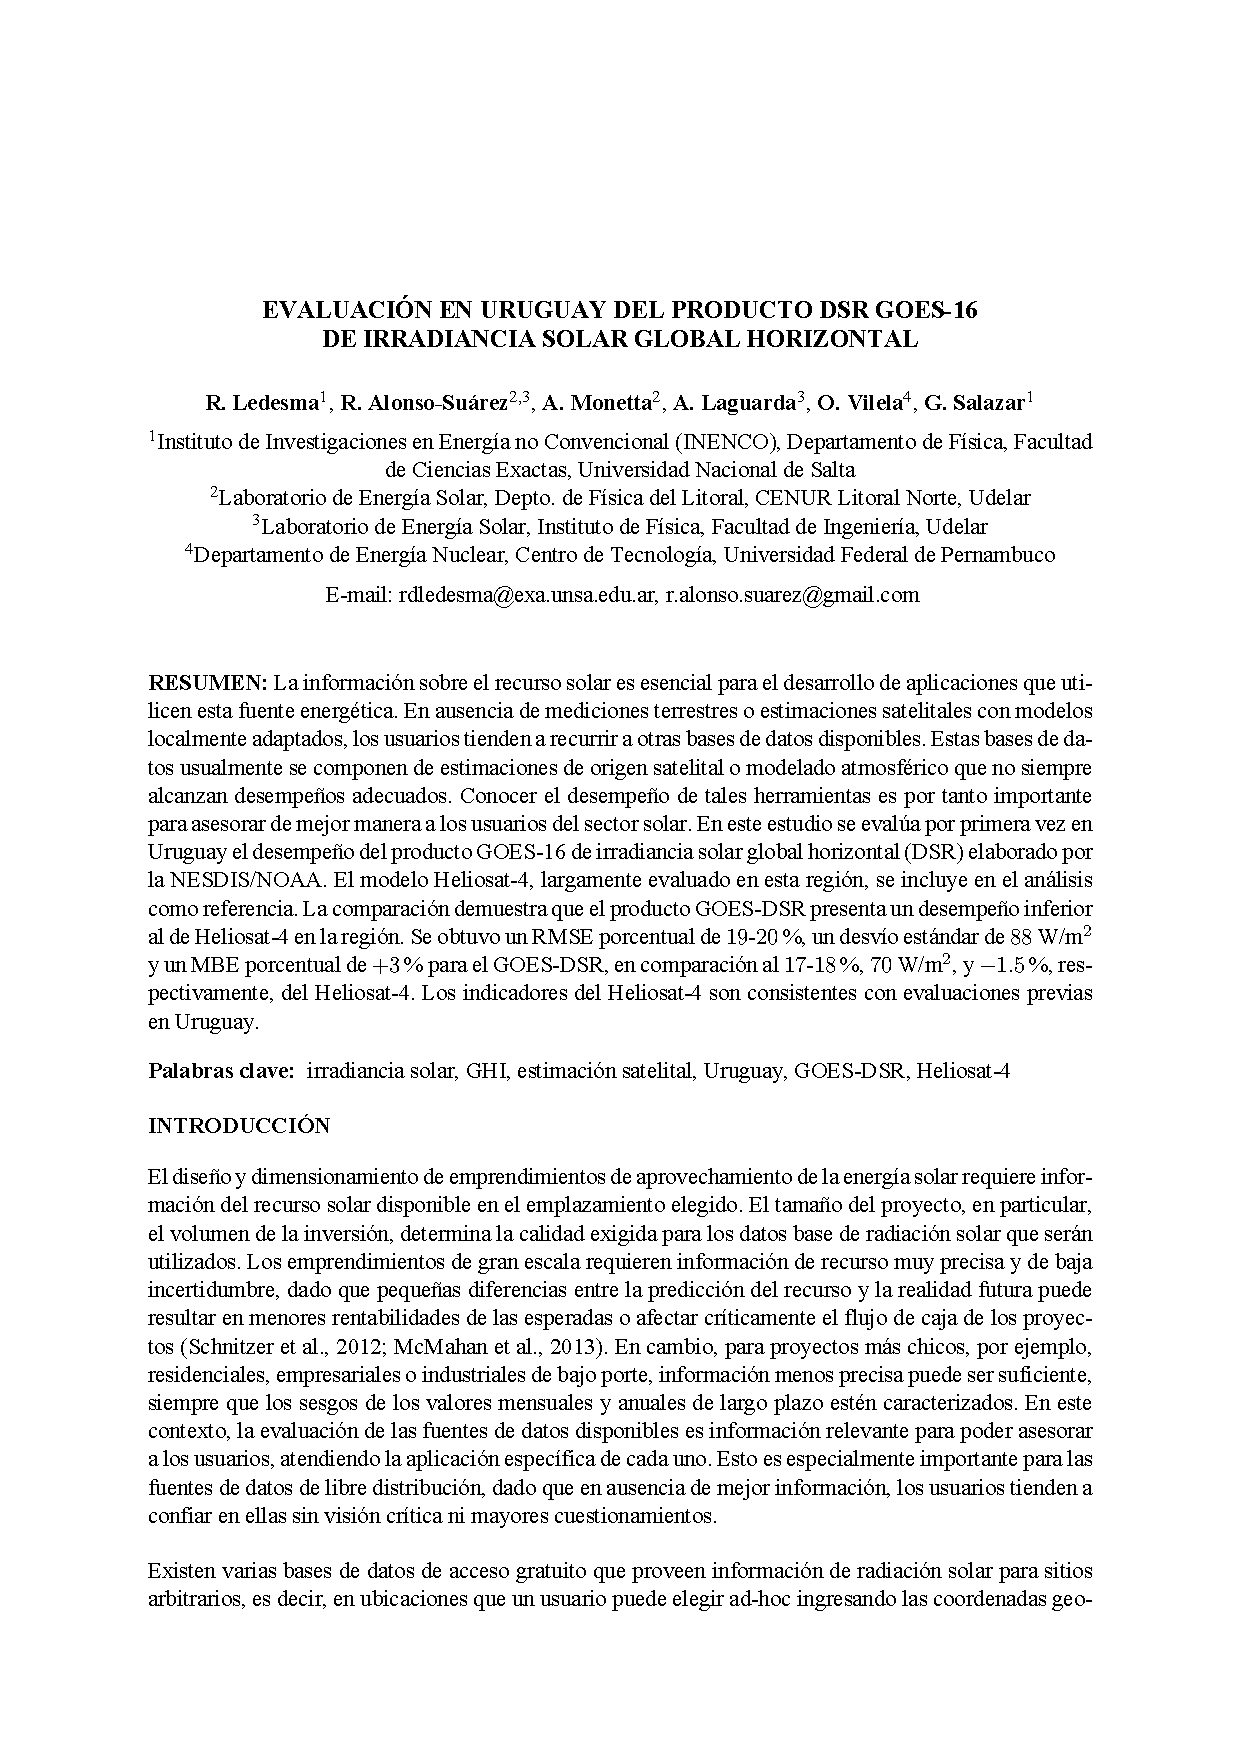
\includepdf[pages=-]{anexo_3/04_DSR}
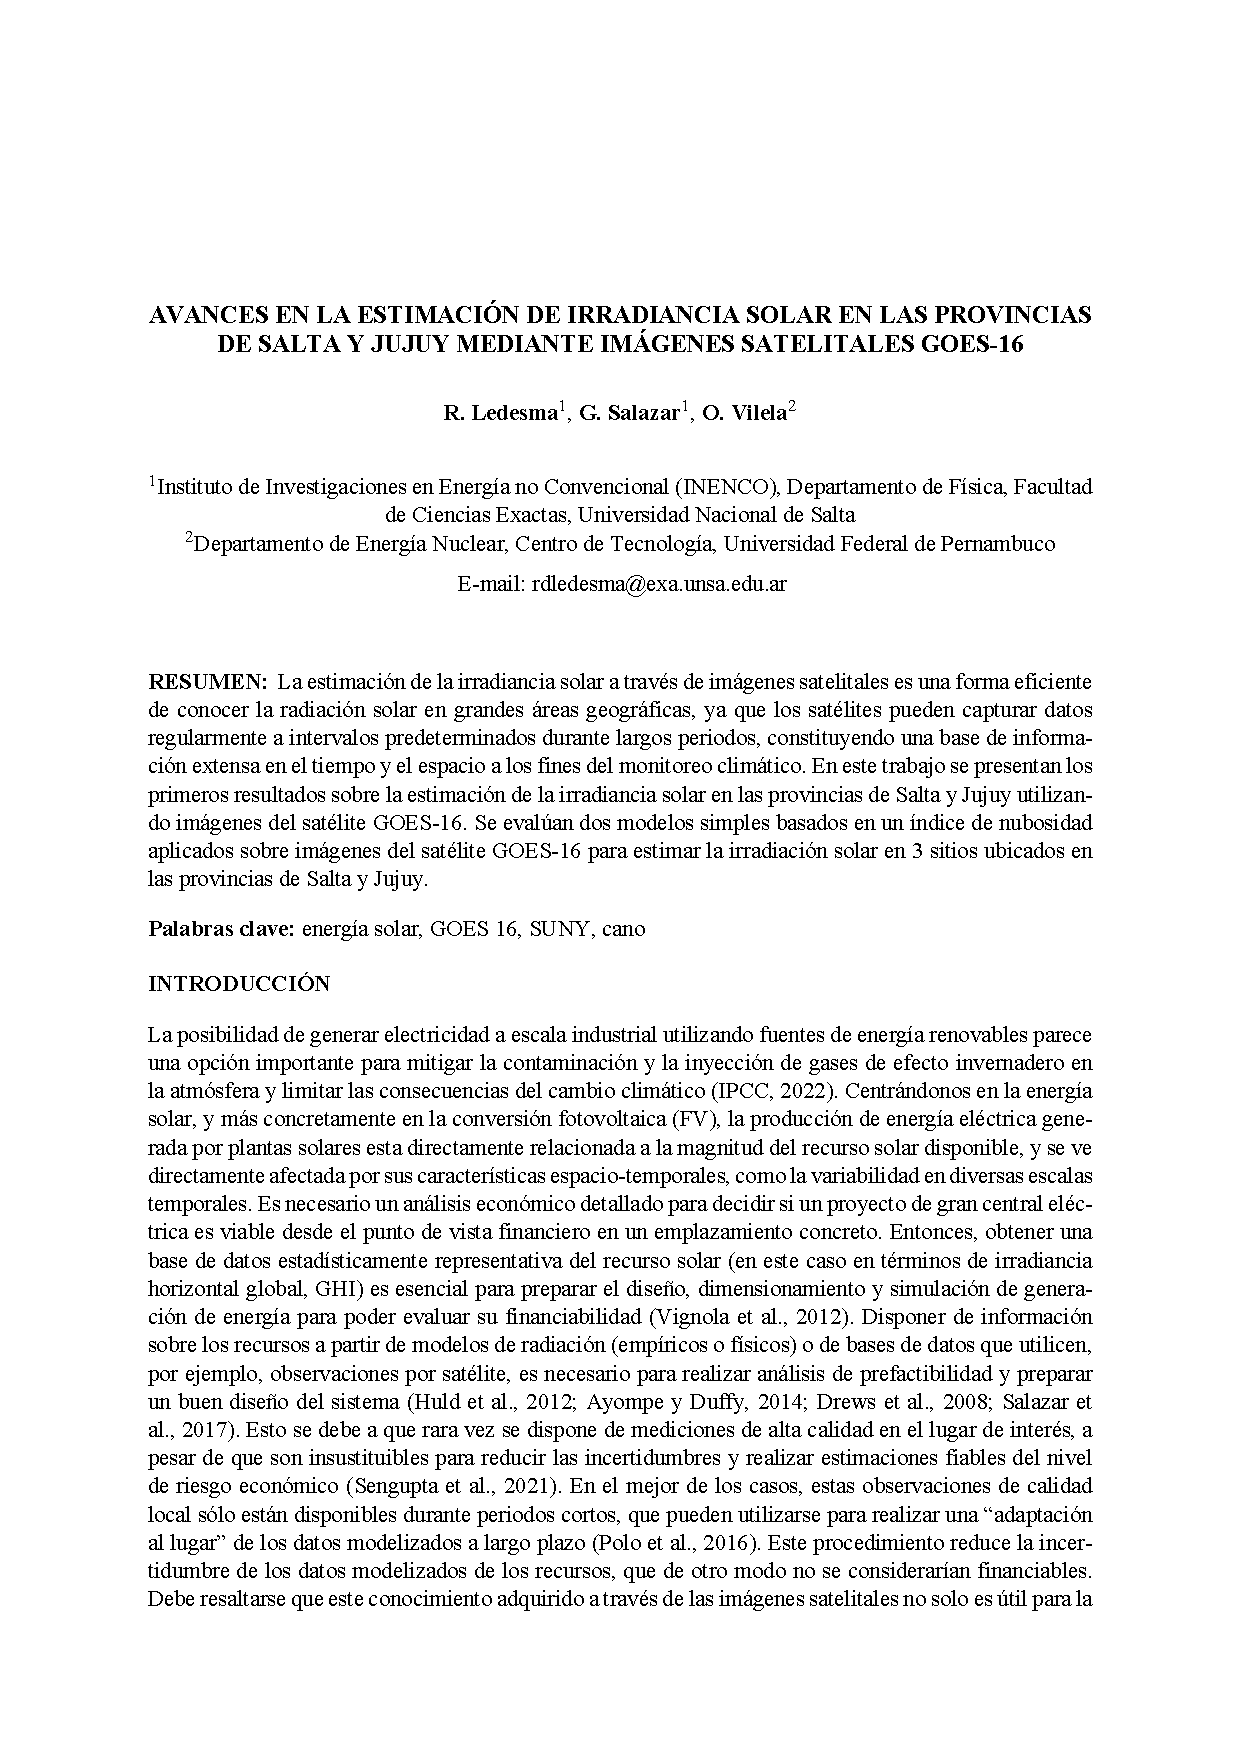
\includepdf[pages=-]{anexo_3/05_GCIM}
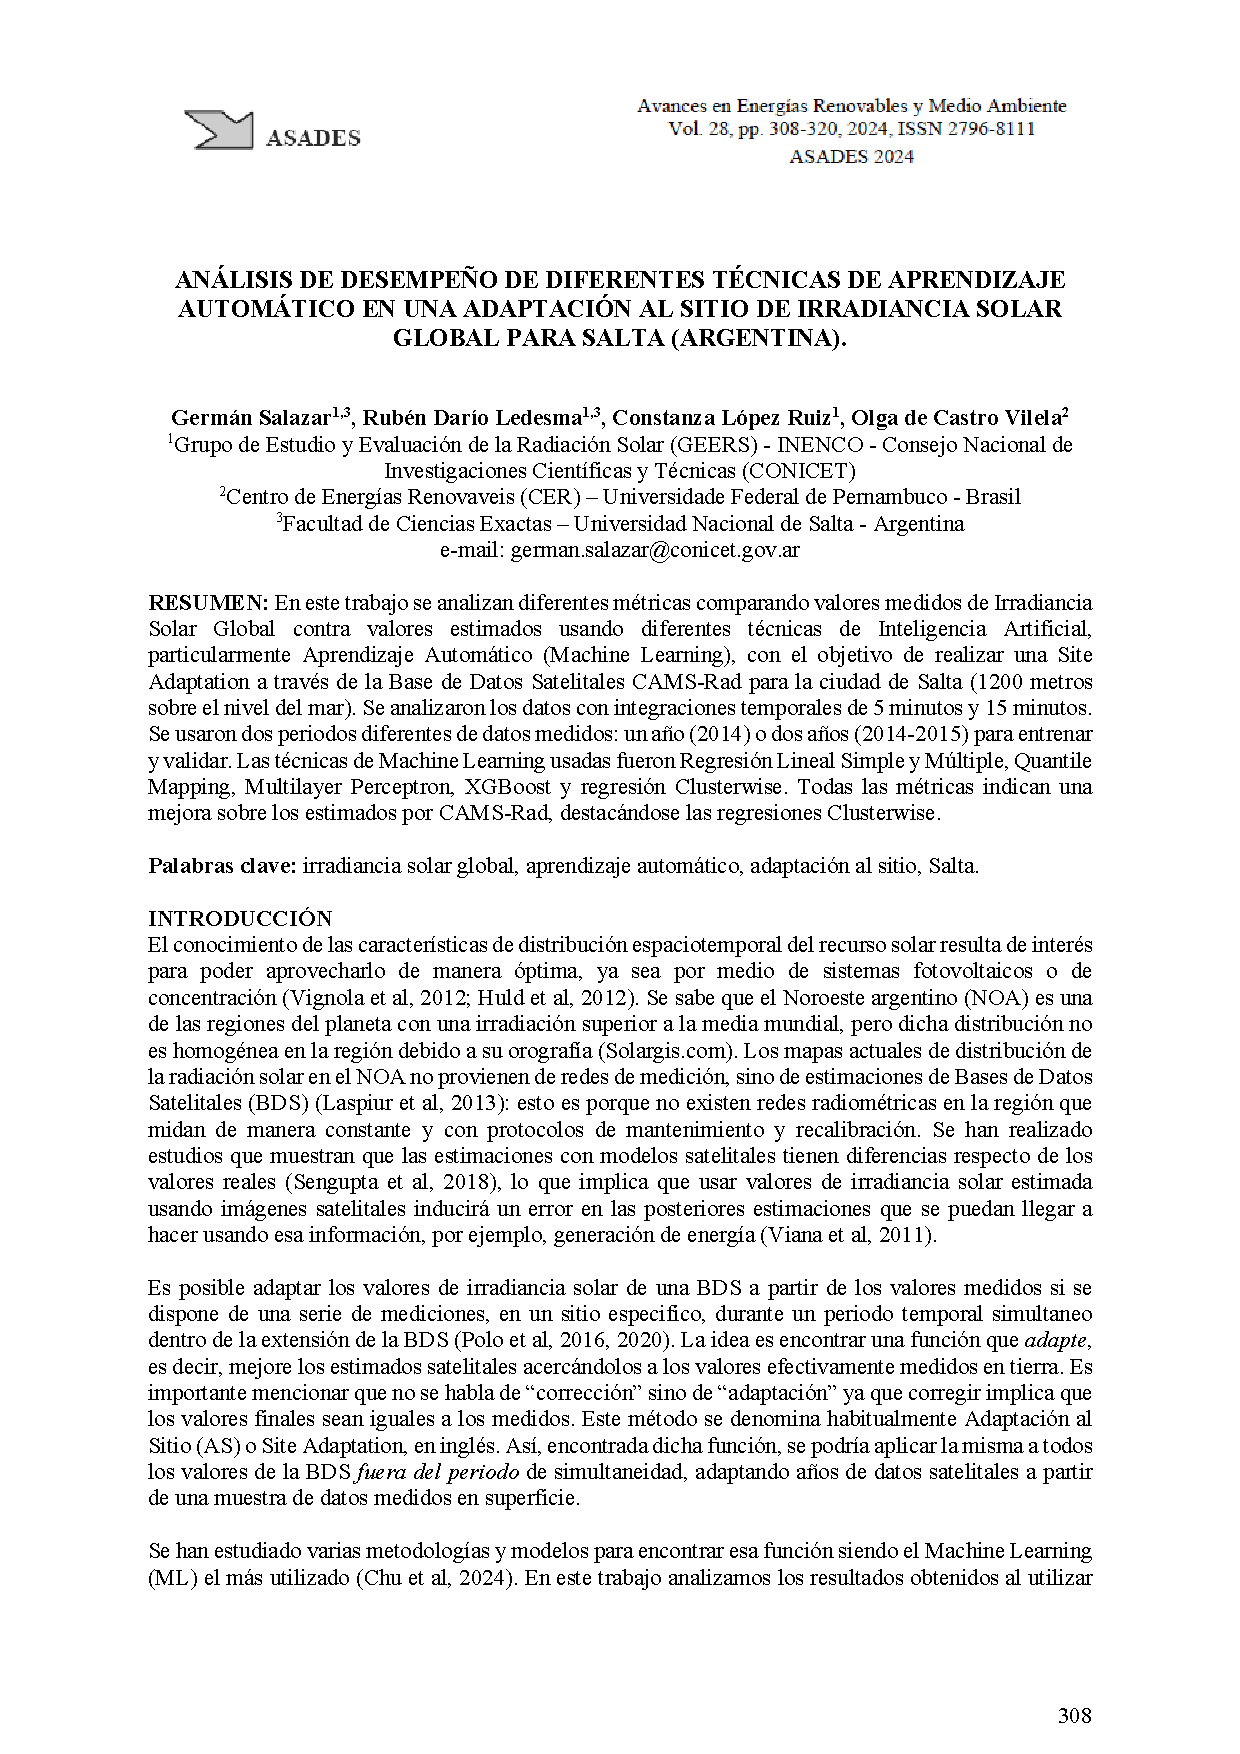
\includepdf[pages=-]{anexo_3/06_DESEMPEÑO}
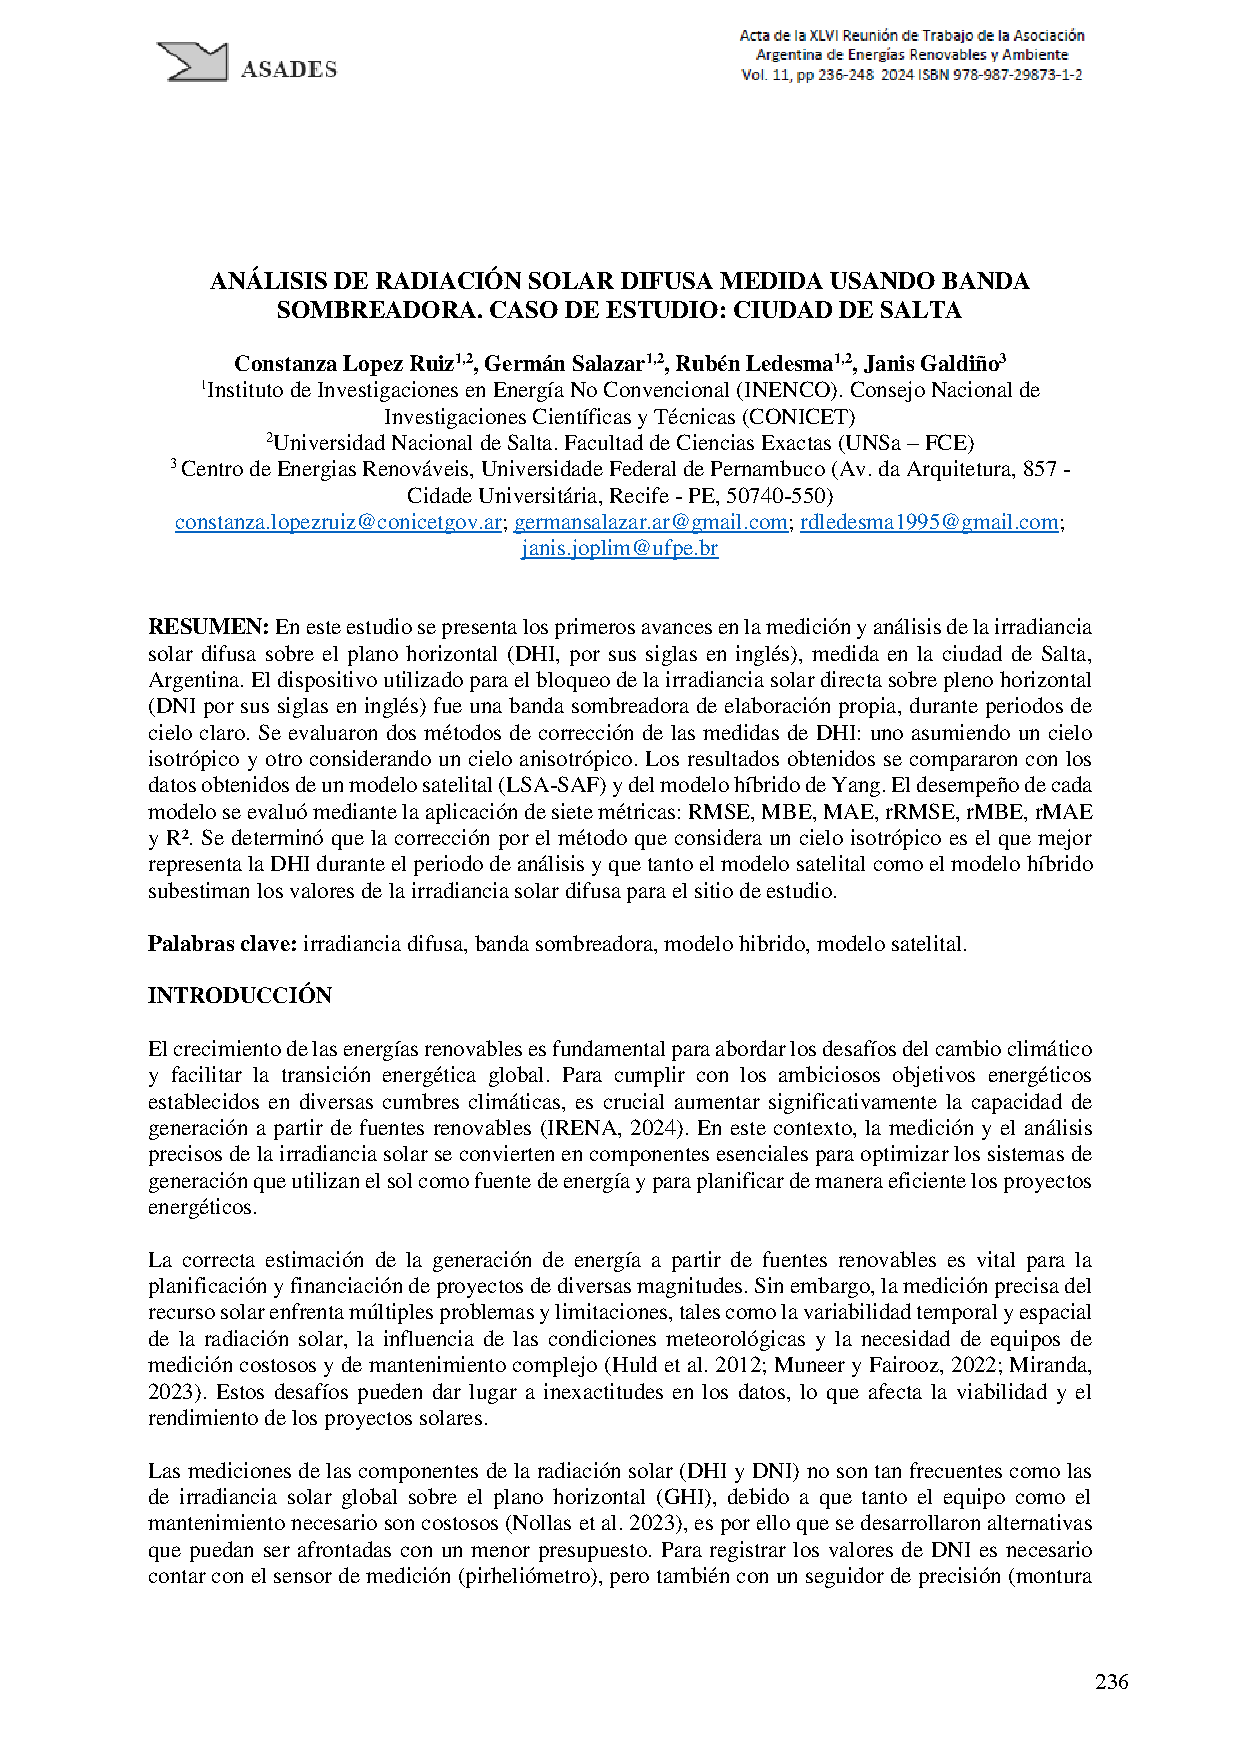
\includepdf[pages=-]{anexo_3/07_DIFUSA}
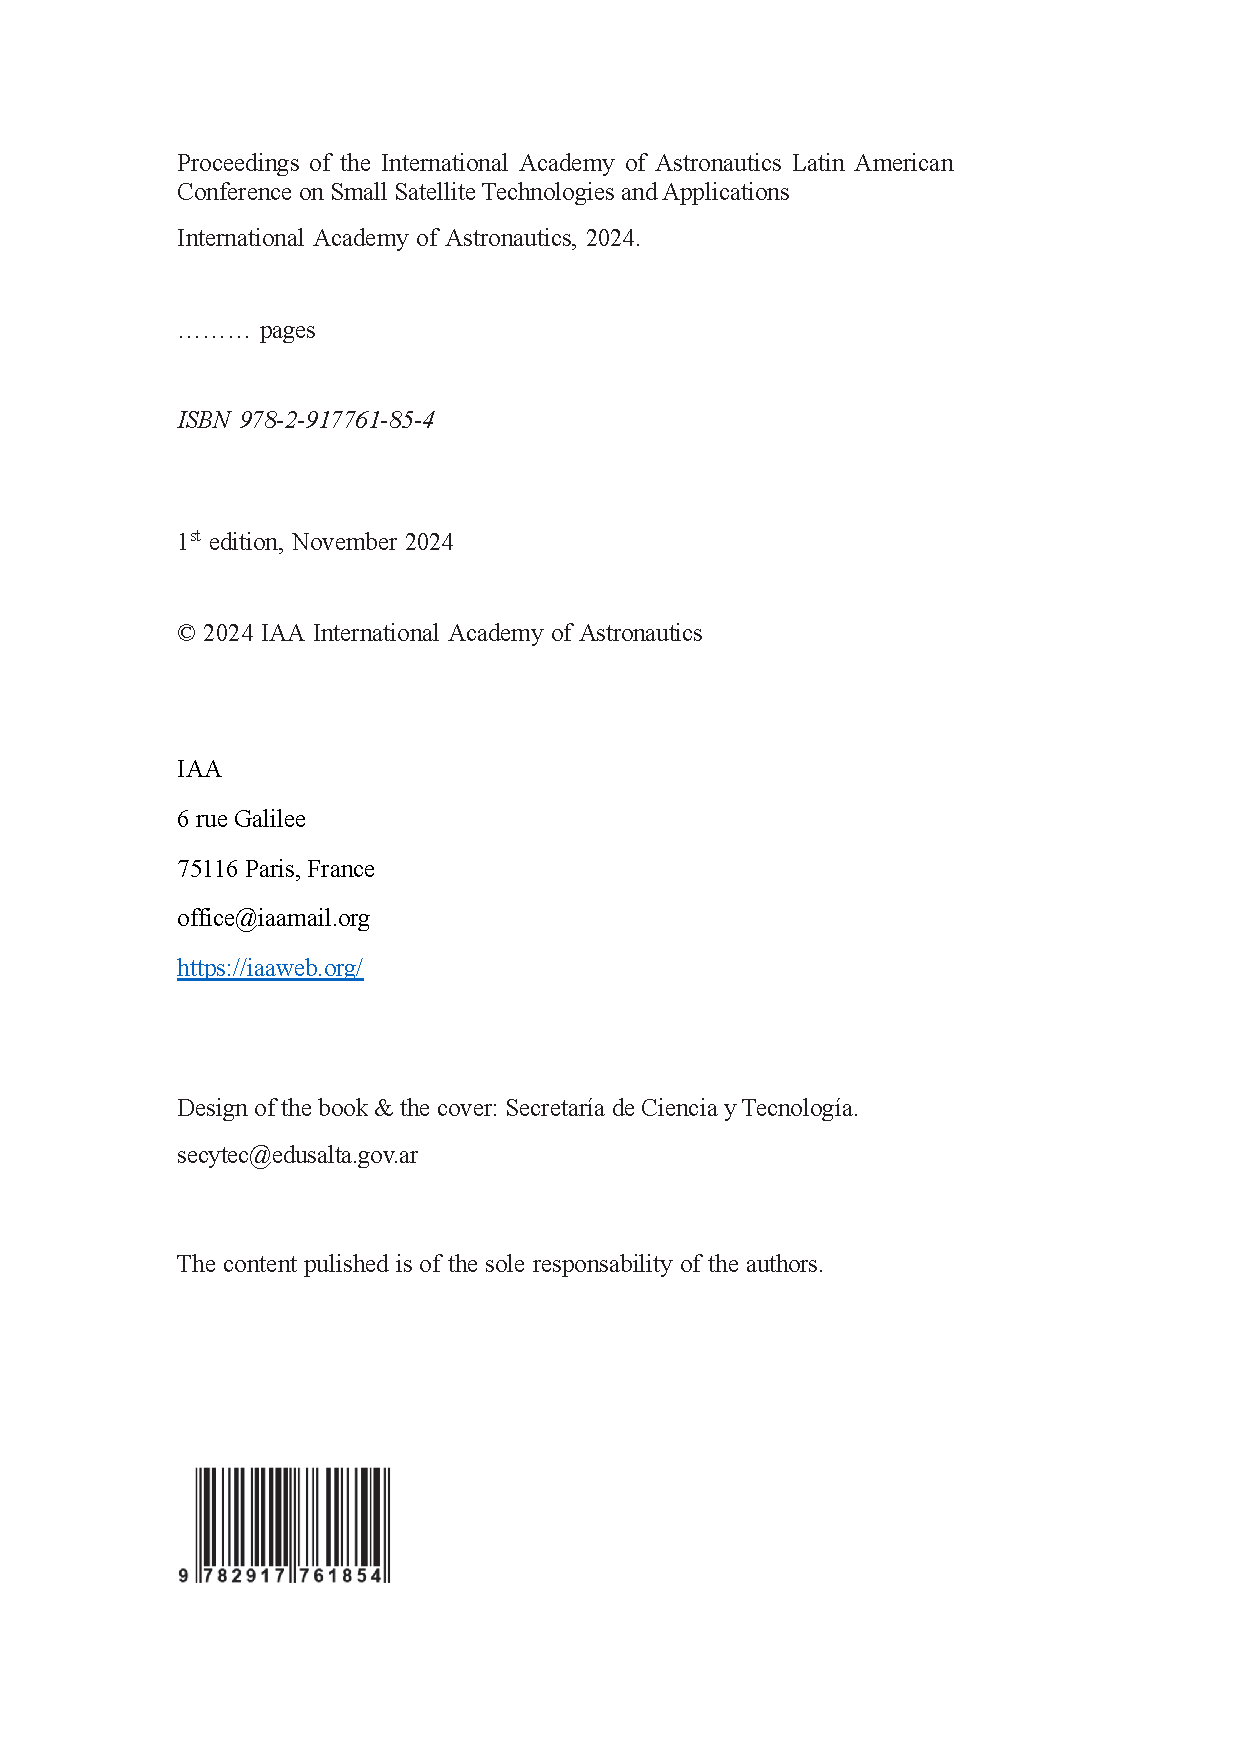
\includepdf[pages=-]{anexo_3/08_small}
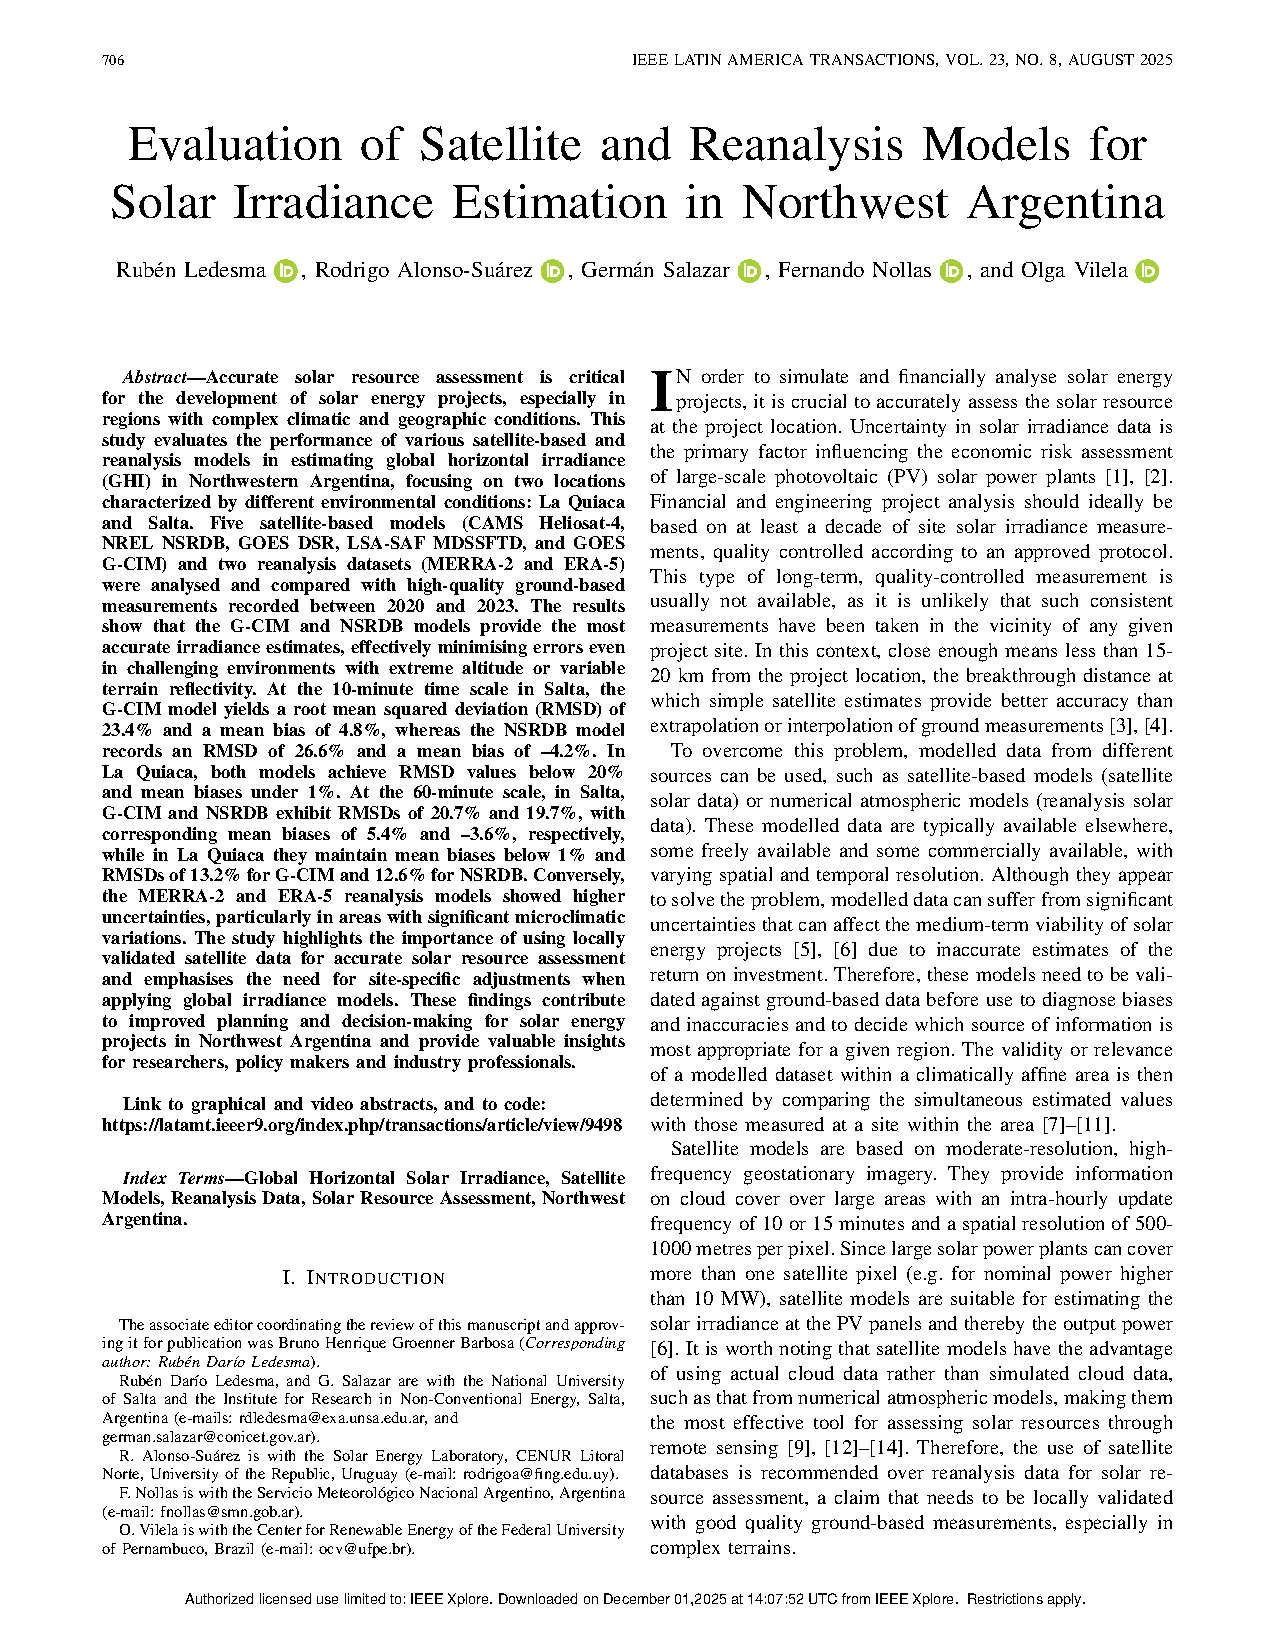
\includepdf[pages=-]{anexo_3/09_IEEE}
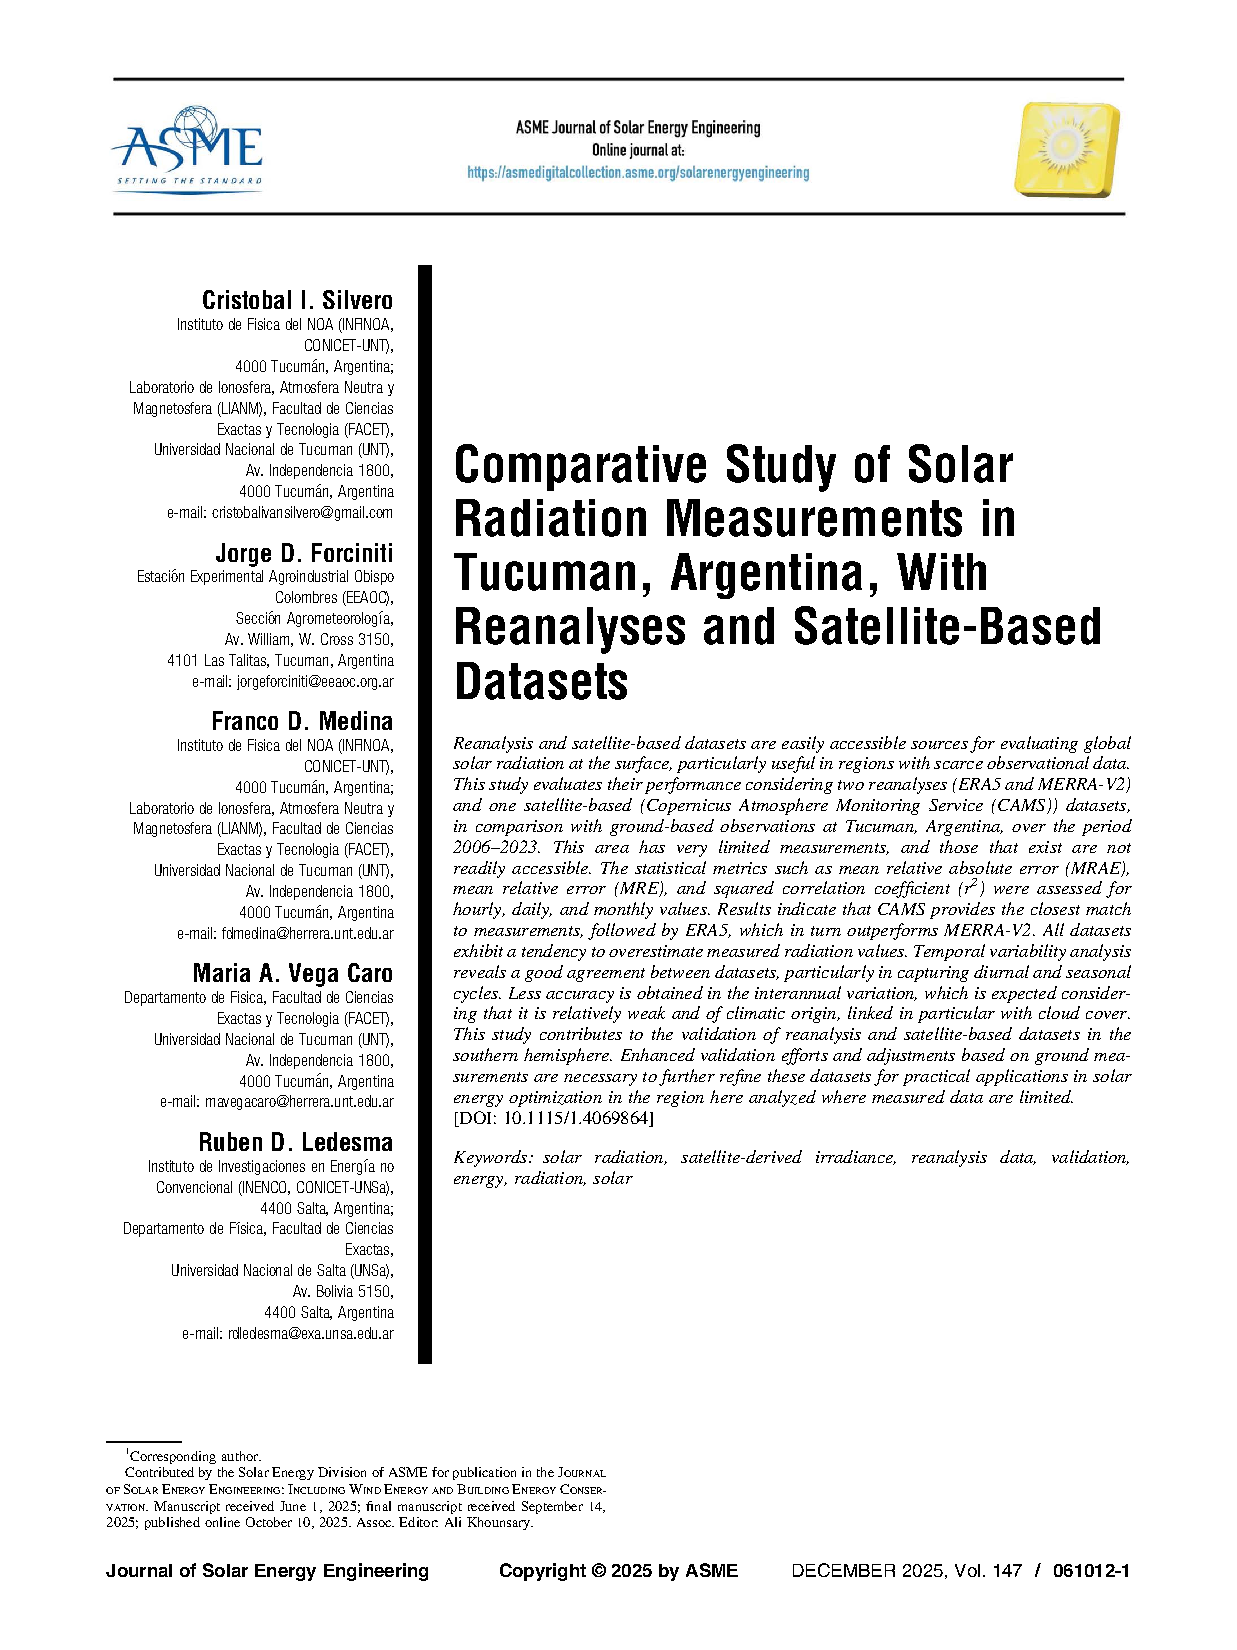
\includepdf[pages=-]{anexo_3/10_SOL}
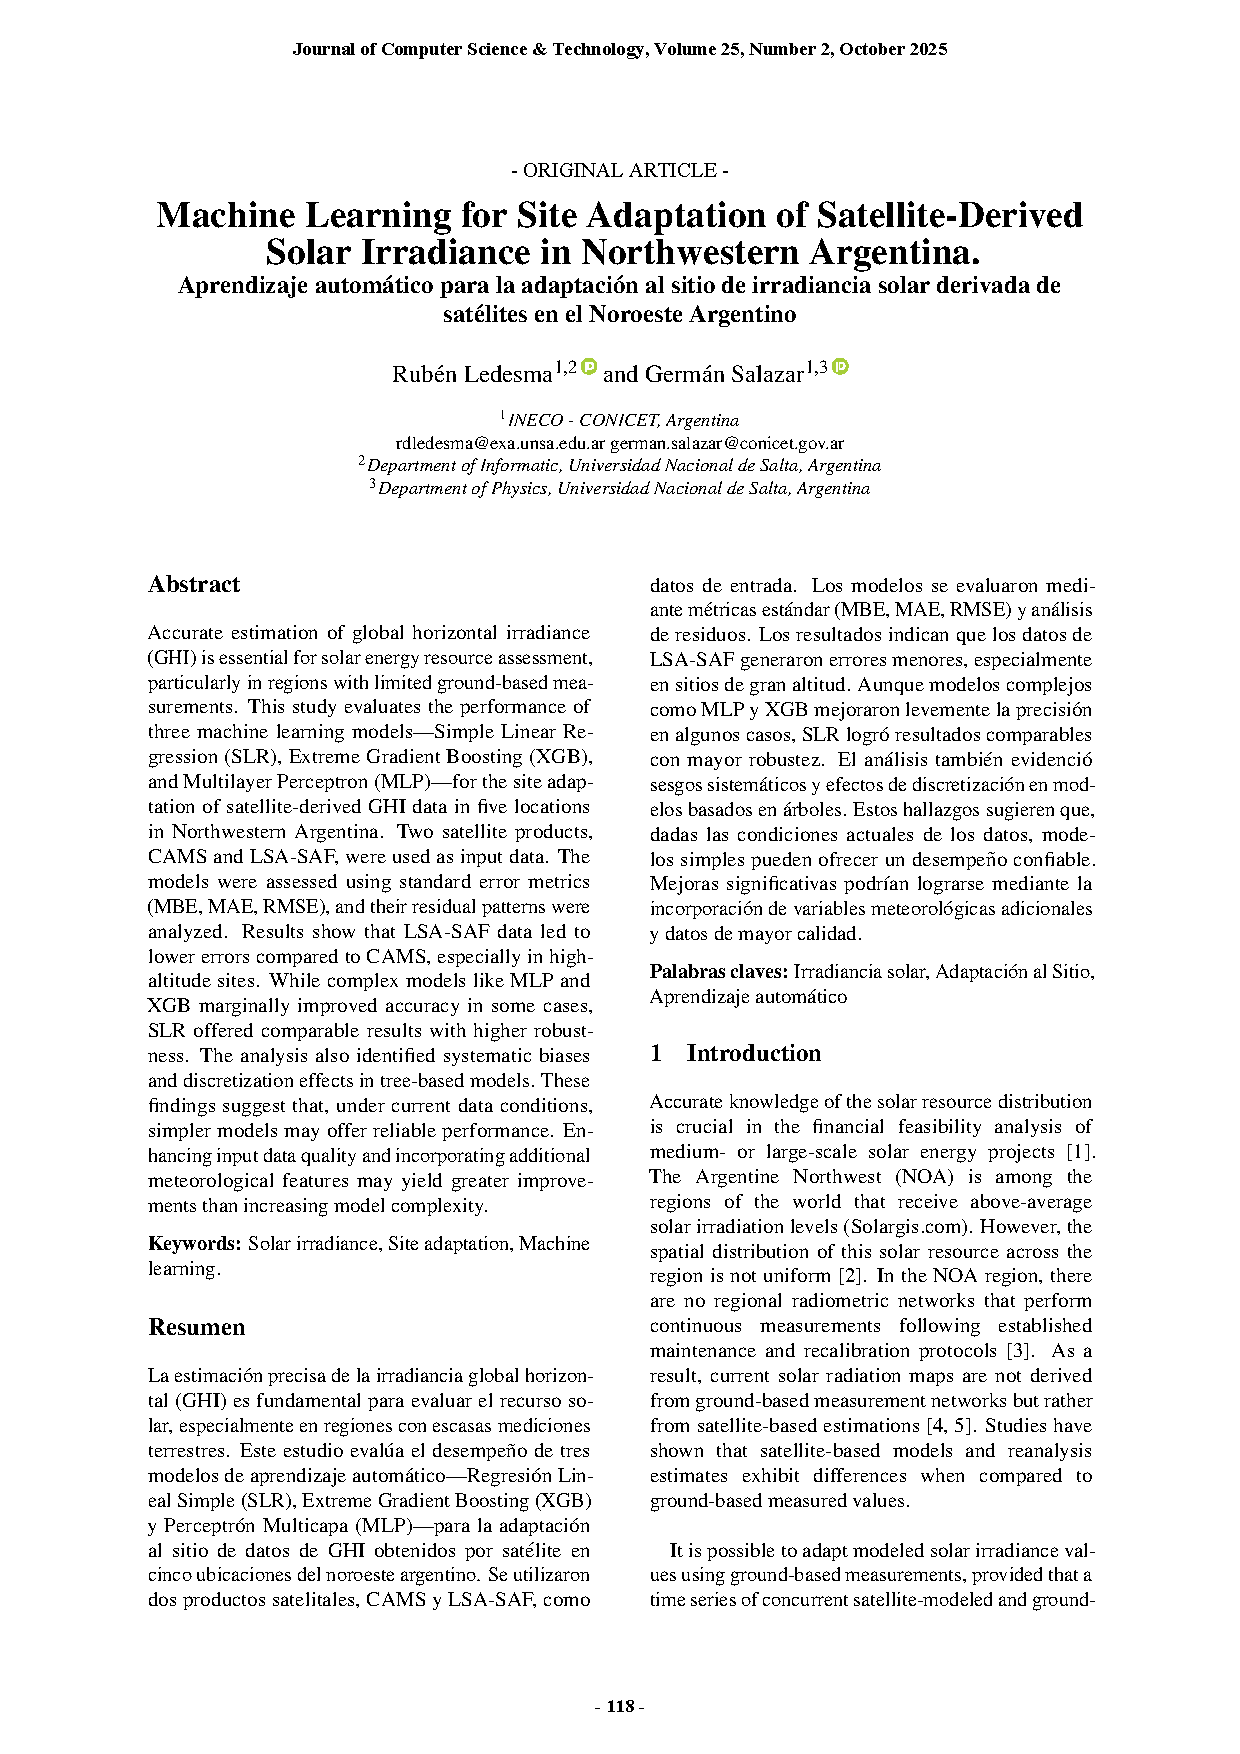
\includepdf[pages=-]{anexo_3/11_ML_JCTS}
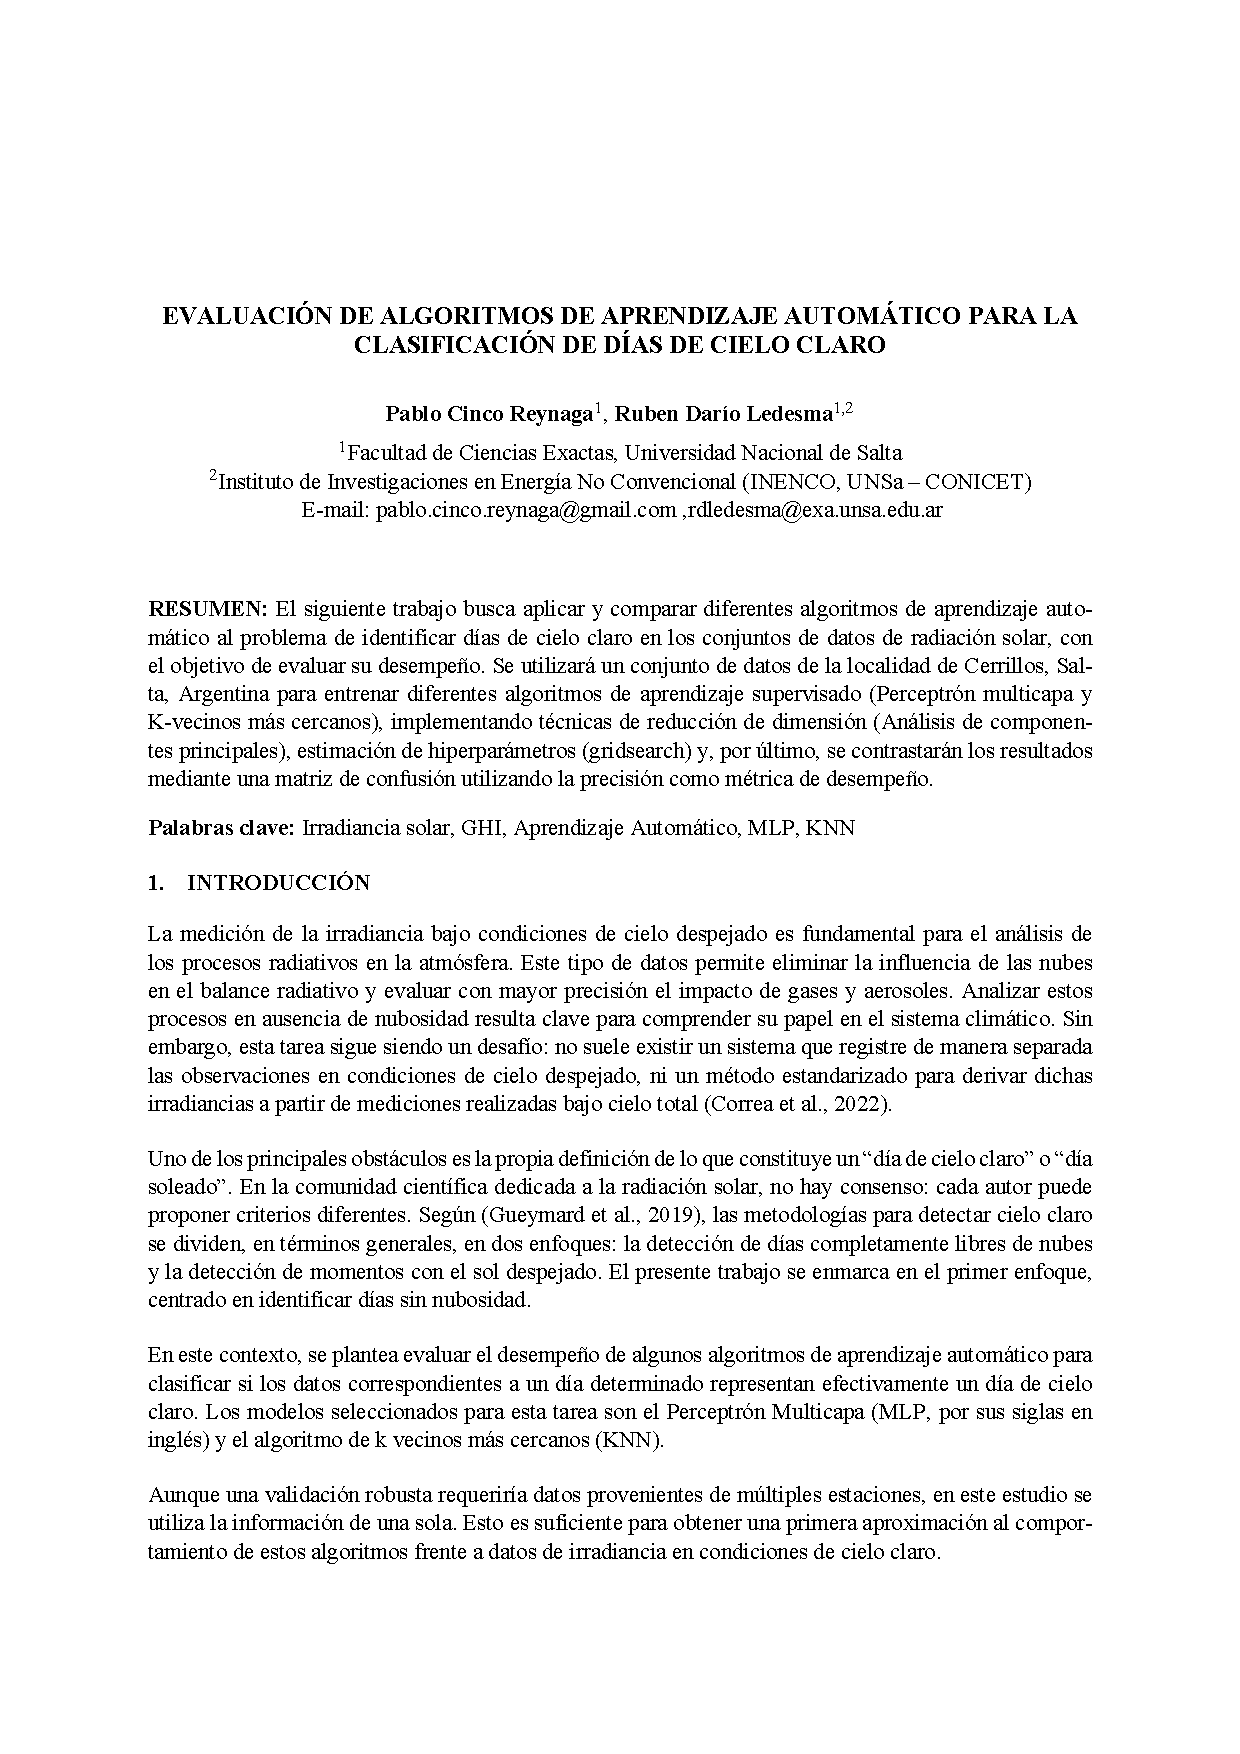
\includepdf[pages=-]{anexo_3/12_Cinco}










